\chapter{Security}

\section{Deleting a struct with mapping} \label{apx:security:mapping}

Slither provides a module for detecting a vulnerability which involves deleting a \texttt{struct} which contains a \texttt{mapping}. We provide an example of a smart contract with this flaw in Figure \ref{fig:mapping-struct}. The steps to reproduce the vulnerability are the following:

\begin{enumerate}
    \item Create a balance for a user by calling \texttt{createBalance(idx)}, let \texttt{idx} be \texttt{42}.
    \item Set the balance of a target address to a value, let the address be \texttt{0x1} and the value \texttt{100}.
    \item Delete the balance by calling \texttt{deleteBalance(42)}. It is expected that the \texttt{struct} at the index 42 will be deleted, along with all its contents.
    \item Create a balance for another user by calling \texttt{createBalance(42)}. Retrieving that user's balance it can be seen that it is 100, instead of the expected 0.
\end{enumerate}

\begin{figure}[htb]
    \centering
    \lstinputlisting[language=Solidity]{contracts/Bank.sol}
    \caption{Mapping inside a struct}
    \label{fig:mapping-struct}
\end{figure}

\section{Honeypot Smart Contracts} \label{honeypots}

Since the second Parity bug no novel critical vulnerabilities have been identified in smart contracts. However, smart contracts that are architected to look vulnerable to known exploits started surfacing, with their true goal being to steal the funds of potential hackers. Hackers who attempt to exploit them need to first deposit some amount of ether before trying to drain the contract. Each honeypot has a mechanism to prevent the attacker from draining any funds. As a result, only the contract owner is able to withdraw the balance of the contract, including any stolen amounts. We proceed to describe the functionality of a honeypot which takes advantage of `Variable Shadowing' in Solidity. 

The contract in Figure \ref{fig:owner_honeypot} was deployed with an initial amount of 0.1 ether as a balance. At first, it seems that an adversary can send an amount of ether to the smart contract, and due to the fallback function\footnote{A fallback function is a unnamed function which gets called when a call is made to a smart contract that does not match any of its function signatures, or when ether is send to the contract's address.}, if the amount is larger than the value of \texttt{jackpot} the \texttt{owner} variable will be changed to the attacker's address. After that, the adversary should be able to call \texttt{takeAll} and withdraw the funds from the contract.

\begin{figure}[ht!]
    \centering
    \lstinputlisting[language=Solidity]{contracts/var_shadow.sol}
    \caption{A honeypot which takes advantage of Variable Shadowing.}
    \label{fig:owner_honeypot}
\end{figure}

\begin{figure}[ht!]
    \centering
    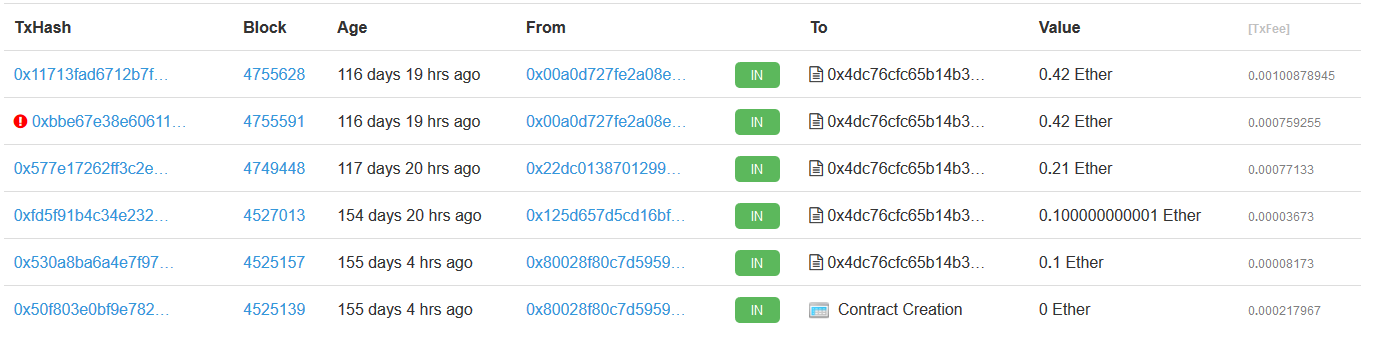
\includegraphics[width=\textwidth]{honeypot}
    \caption{Transactions trying to get ownership of the honeypot contract}
    \label{fig:honeypot_tx}
\end{figure}

Users tried to exploit it by depositing funds and expecting the ownership to change to their address so that they would be able to withdraw the contract's funds. Contrary to what is expected, after sending enough ether to the contract, the \texttt{owner} variable which gets changed belongs to \texttt{KingOfTheHill} contract. The \texttt{takeAll} function, is decorated by the \texttt{onlyOwner} modifier\footnote{A modifier is a special function which gets executed before or after the function it \textit{modifies}. They are primarily used to enforce access control in functions.} which looks for the value of \texttt{owner} in the \texttt{Owned} contract. As a result, the `real' \texttt{owner} of the contract is unchanged, and the attacker is unable to claim ownership, effectively losing their funds. Running Slither on the contract can reveal the variable shadowing as shown in \ref{fig:slither_shadowing}.

\begin{figure}[H]
    \centering
    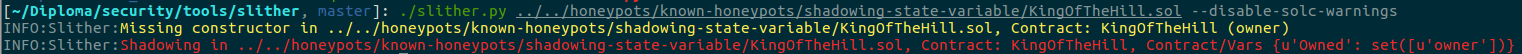
\includegraphics[width=\textwidth]{slither_shadowing}
    \caption{Slither is able to detect the variable shadowing in \texttt{owner}}
    \label{fig:slither_shadowing}
\end{figure}